\documentclass[../../../main.tex]{subfiles}
\begin{document}

%%%%%%%%%%%%%%%%%%%%%%%%%%%%%%%%%%%%%%%%%
%%%%%%%%%%%%%%%%%%%%%%%%%%%%%%%%%%%%%%%%%
%%%%%%%%%%%%%%%%%%%%%%%%%%%%%%%%%%%%%%%%%
\chapter{Type I Errors}


There are two kinds of errors we can make when testing a hypothesis in the way we are discussing now. The first is called a \vocab{Type I Error}, and the second is called a \vocab{Type II Error}. 

Let's talk about Type I Errors first. This kind of error occurs when we (mistakenly) reject a good null hypothesis. How does this happen?


%%%%%%%%%%%%%%%%%%%%%%%%%%%%%%%%%%%%%%%%%
%%%%%%%%%%%%%%%%%%%%%%%%%%%%%%%%%%%%%%%%%
\section{No Type I Errors}

To start, let us consider a case where Type I Errors cannot happen. Consider the example from before. The null hypothesis proposes that $\HypPopMean/$ is 55K, and the claim is that the true population mean $\populationmean$ is greater than or equal to that. 

Suppose also that the sampling distributions have a spread that spans a stretch of 10K. So, if the true population mean rests at 55, then the normal sampling curve that's centered on that will extend 5K to the left, and 5K to the right (i.e., from 50K to 60K):

\begin{center}
  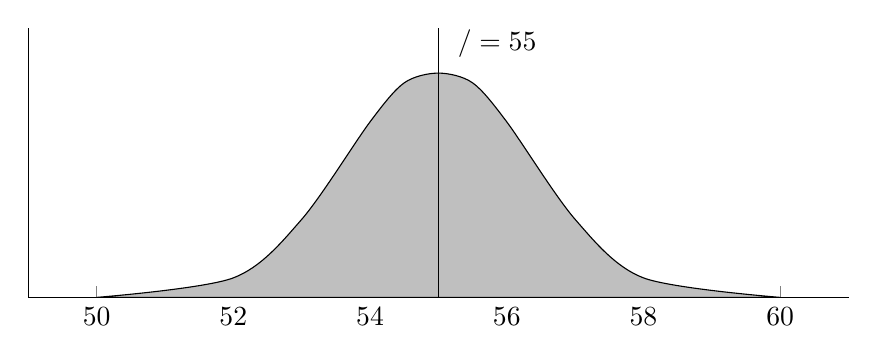
\begin{tikzpicture}
    \begin{axis}[
      axis lines*=left,
      ytick=\empty,
      height=5cm,
      width=12cm,
      enlarge y limits={value=0.2,upper},
      ]
      \addplot[smooth, fill=lightgray, domain=45:65] 
        coordinates{
          (50, 0) (52, 0.5) (53, 2) (54, 4.5) (54.5, 5.5)
          (55, 5.75)
          (55.5, 5.5) (56, 4.5) (57, 2) (58, 0.5) (60, 0)} 
        \closedcycle;

      \draw (55, 0) -- (55, 10);
      \node at (55, 6.5) [label=right:{$\HypPopMean/ = 55$}] {};

    \end{axis}
  \end{tikzpicture}
\end{center}

\noindent
Now, suppose that we set our critical point ($\alpha$) at the far left edge of this sampling distribution, i.e., exactly at 50:

\begin{center}
  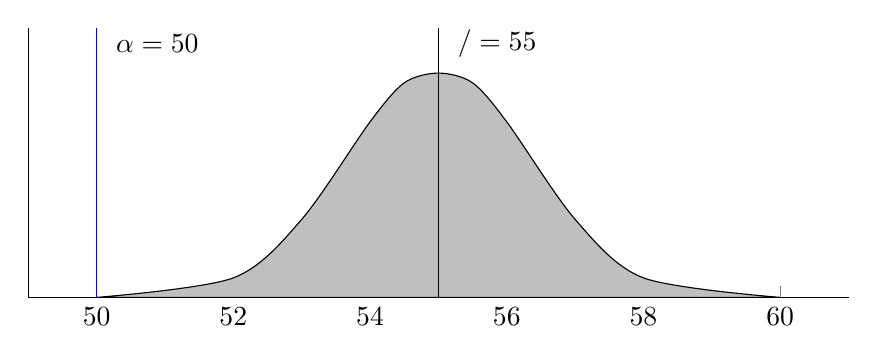
\begin{tikzpicture}
    \begin{axis}[
      axis lines*=left,
      ytick=\empty,
      height=5cm,
      width=12cm,
      enlarge y limits={value=0.2,upper},
      ]
      \addplot[smooth, fill=lightgray, domain=45:65] 
        coordinates{
          (50, 0) (52, 0.5) (53, 2) (54, 4.5) (54.5, 5.5)
          (55, 5.75)
          (55.5, 5.5) (56, 4.5) (57, 2) (58, 0.5) (60, 0)} 
        \closedcycle;

      \draw (55, 0) -- (55, 10);
      \node at (55, 6.5) [label=right:{$\HypPopMean/ = 55$}] {};

      \draw[color=blue] (50, 0) -- (50, 10);
      \node at (50, 6.5) [label=right:{$\alpha = 50$}] {};

    \end{axis}
  \end{tikzpicture}
\end{center}

\noindent
By doing that, we're saying that we are not going to reject the null hypothesis, unless we get a sample mean that is lower than this value. If we get any sample mean that is higher than $\alpha$, we will let the null hypothesis stand.

Think about this. In order to make a Type I Error, we need to reject the null hypothesis. I mean, you can't be mistaken about rejecting something, if you never reject it. So, if we want to commit a Type I Error, we need to first reject the null hypothesis, and then be mistaken about it. What this means is that, if we get a sample mean that is anywhere to the right of $\alpha$, we won't reject the null hypothesis, in which case we can't be mistaken about rejecting it, and so we cannot commit a Type I Error.

Hence, we can take that curve that is centered on 55K, and slide it anywhere to the right. For example:

\begin{center}
  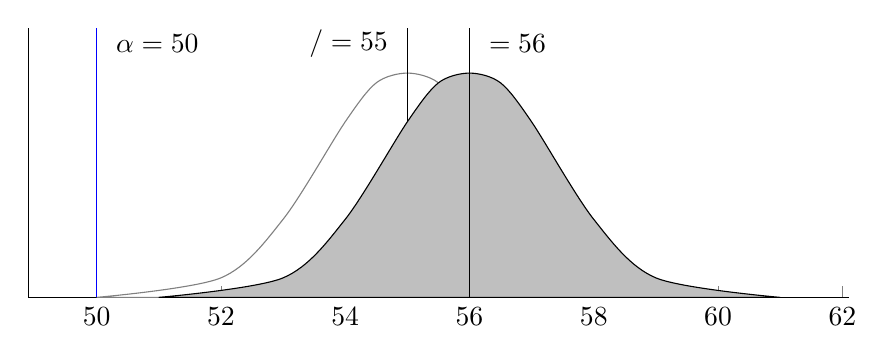
\begin{tikzpicture}
    \begin{axis}[
      axis lines*=left,
      ytick=\empty,
      height=5cm,
      width=12cm,
      enlarge y limits={value=0.2,upper},
      ]
      \addplot[smooth, color=gray, domain=45:65] 
        coordinates{
          (50, 0) (52, 0.5) (53, 2) (54, 4.5) (54.5, 5.5)
          (55, 5.75)
          (55.5, 5.5) (56, 4.5) (57, 2) (58, 0.5) (60, 0)} 
        \closedcycle;

      \draw (55, 0) -- (55, 10);
      \node at (55, 6.5) [label=left:{$\HypPopMean/ = 55$}] {};

      \draw[color=blue] (50, 0) -- (50, 10);
      \node at (50, 6.5) [label=right:{$\alpha = 50$}] {};

      \addplot[smooth, fill=lightgray, domain=45:65] 
        coordinates{
          (51, 0) (53, 0.5) (54, 2) (55, 4.5) (55.5, 5.5)
          (56, 5.75)
          (56.5, 5.5) (57, 4.5) (58, 2) (59, 0.5) (61, 0)} 
        \closedcycle;

      \draw (56, 0) -- (56, 10);
      \node at (56, 6.5) [label=right:{$\populationmean = 56$}] {};

    \end{axis}
  \end{tikzpicture}
\end{center}

\noindent
Any sample mean we get from this will be to the right of $\alpha$. For example, a sample mean of 53:

\begin{center}
  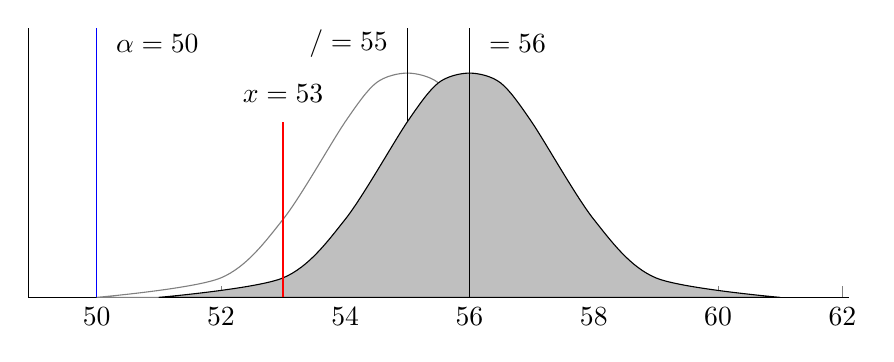
\begin{tikzpicture}
    \begin{axis}[
      axis lines*=left,
      ytick=\empty,
      height=5cm,
      width=12cm,
      enlarge y limits={value=0.2,upper},
      ]
      \addplot[smooth, color=gray, domain=45:65] 
        coordinates{
          (50, 0) (52, 0.5) (53, 2) (54, 4.5) (54.5, 5.5)
          (55, 5.75)
          (55.5, 5.5) (56, 4.5) (57, 2) (58, 0.5) (60, 0)} 
        \closedcycle;

      \draw (55, 0) -- (55, 10);
      \node at (55, 6.5) [label=left:{$\HypPopMean/ = 55$}] {};

      \draw[color=blue] (50, 0) -- (50, 10);
      \node at (50, 6.5) [label=right:{$\alpha = 50$}] {};

      \addplot[smooth, fill=lightgray, domain=45:65] 
        coordinates{
          (51, 0) (53, 0.5) (54, 2) (55, 4.5) (55.5, 5.5)
          (56, 5.75)
          (56.5, 5.5) (57, 4.5) (58, 2) (59, 0.5) (61, 0)} 
        \closedcycle;

      \draw (56, 0) -- (56, 10);
      \node at (56, 6.5) [label=right:{$\populationmean = 56$}] {};

      \draw[color=red] (53, 0) -- (53, 4.5);
      \node at (53, 4.5) [label=above:{$\samplemean{x} = 53$}] {};

    \end{axis}
  \end{tikzpicture}
\end{center}

\noindent
Since this sample mean is on the right side of $\alpha$, we won't reject the null hypothesis. We'll let it stand. 

The true population can keep sliding to the right, and the same will hold good. For example, if the true population mean is over at 60, any sample we get in that sampling distribution will be to the right of $\alpha$, so we won't reject the null hypothesis:

\begin{center}
  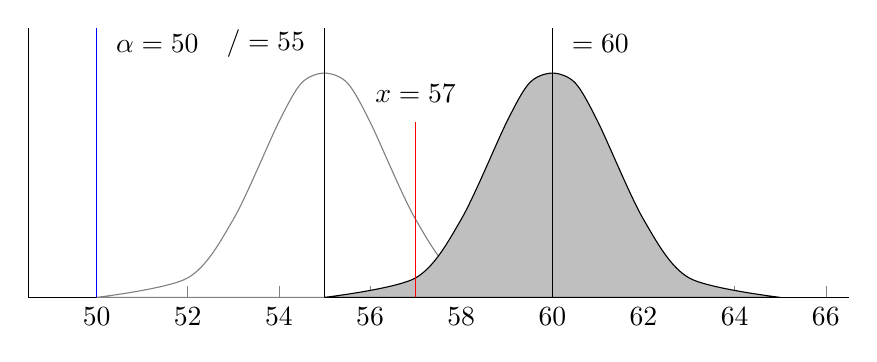
\begin{tikzpicture}
    \begin{axis}[
      axis lines*=left,
      ytick=\empty,
      height=5cm,
      width=12cm,
      enlarge y limits={value=0.2,upper},
      ]
      \addplot[smooth, color=gray, domain=45:65] 
        coordinates{
          (50, 0) (52, 0.5) (53, 2) (54, 4.5) (54.5, 5.5)
          (55, 5.75)
          (55.5, 5.5) (56, 4.5) (57, 2) (58, 0.5) (60, 0)} 
        \closedcycle;

      \draw (55, 0) -- (55, 10);
      \node at (55, 6.5) [label=left:{$\HypPopMean/ = 55$}] {};

      \draw[color=blue] (50, 0) -- (50, 10);
      \node at (50, 6.5) [label=right:{$\alpha = 50$}] {};

      \addplot[smooth, fill=lightgray, domain=45:65] 
        coordinates{
          (55, 0) (57, 0.5) (58, 2) (59, 4.5) (59.5, 5.5)
          (60, 5.75)
          (60.5, 5.5) (61, 4.5) (62, 2) (63, 0.5) (65, 0)} 
        \closedcycle;

      \draw (60, 0) -- (60, 10);
      \node at (60, 6.5) [label=right:{$\populationmean = 60$}] {};

      \draw[color=red] (57, 0) -- (57, 4.5);
      \node at (57, 4.5) [label=above:{$\samplemean{x} = 57$}] {};

    \end{axis}
  \end{tikzpicture}
\end{center}

\noindent
So we can't commit a Type I Error in any of these cases, because we won't reject the null hypothesis in any of theses cases. 

The only way we can commit a Type I Error is to reject the null hypothesis, and be mistaken about it. But the only scenario where we will reject the null hypothesis, is the scenario where we get a sample mean that falls to the \emph{left} of $\alpha$. So we need a sample mean smaller than $\alpha$ to reject the null hypothesis.

Now, because we've placed $\alpha$ at the far left edge of the sampling distribution where the population mean is 55, the only way we could get a sample mean that is \emph{lower} than $\alpha$, is if it were to come from a population mean that is \emph{lower} than 55K. In other words, we would need to take that curve centered at 55K, and slide it a little to the left, in order to get a sample from it that falls on the left side of $\alpha$.

For example, suppose that the true population mean is centered at 55, and just by chance we get a sample that has a mean of 50.5. So our sample mean is way over on the left tail of the sampling distribution:

\begin{center}
  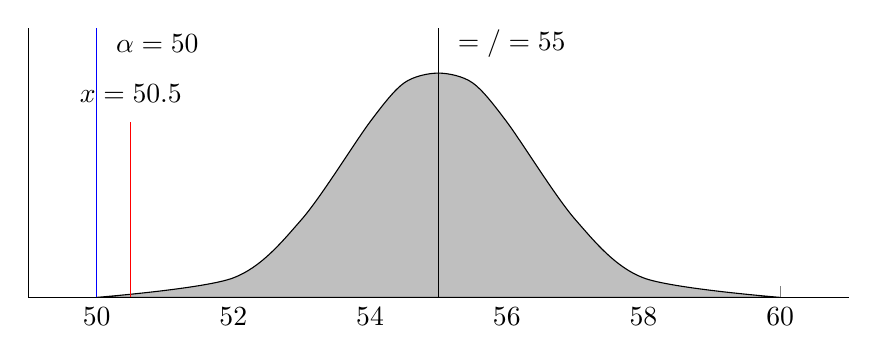
\begin{tikzpicture}
    \begin{axis}[
      axis lines*=left,
      ytick=\empty,
      height=5cm,
      width=12cm,
      enlarge y limits={value=0.2,upper},
      ]
      \addplot[smooth, fill=lightgray, domain=45:65] 
        coordinates{
          (50, 0) (52, 0.5) (53, 2) (54, 4.5) (54.5, 5.5)
          (55, 5.75)
          (55.5, 5.5) (56, 4.5) (57, 2) (58, 0.5) (60, 0)} 
        \closedcycle;

      \draw (55, 0) -- (55, 10);
      \node at (55, 6.5) [label=right:{$\populationmean = \HypPopMean/ = 55$}] {};

      \draw[color=blue] (50, 0) -- (50, 10);
      \node at (50, 6.5) [label=right:{$\alpha = 50$}] {};

      \draw[color=red] (50.5, 0) -- (50.5, 4.5);
      \node at (50.5, 4.5) [label=above:{$\samplemean{x} = 50.5$}] {};

    \end{axis}
  \end{tikzpicture}
\end{center}

\noindent
Nevertheless, the sample mean is still to the \emph{right} of $\alpha$, so we will not reject the null hypothesis.

The only way to get a sample mean on the \emph{left} of $\alpha$ is to slide the population over to the left a little. For example, suppose we slide the true population mean a little to the left (to 54). Then the sample that comes from the far left tail will get pushed just to the left of $\alpha$:

\begin{center}
  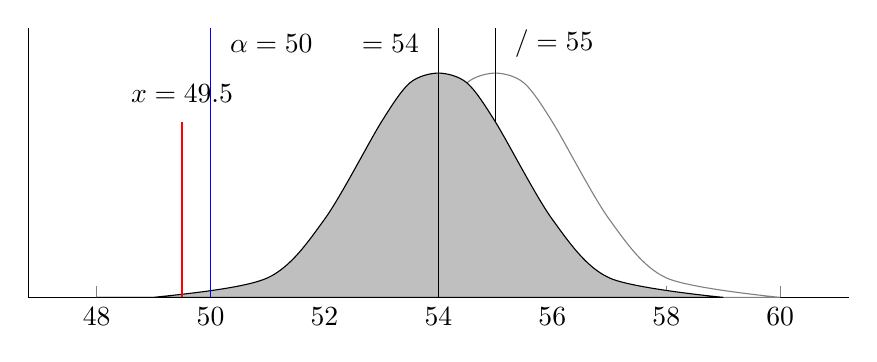
\begin{tikzpicture}
    \begin{axis}[
      axis lines*=left,
      ytick=\empty,
      height=5cm,
      width=12cm,
      enlarge y limits={value=0.2,upper},
      ]
      \addplot[smooth, color=gray, domain=45:65] 
        coordinates{
          (48, 0)
          (50, 0) (52, 0.5) (53, 2) (54, 4.5) (54.5, 5.5)
          (55, 5.75)
          (55.5, 5.5) (56, 4.5) (57, 2) (58, 0.5) (60, 0)} 
        \closedcycle;

      \draw (55, 0) -- (55, 10);
      \node at (55, 6.5) [label=right:{$\HypPopMean/ = 55$}] {};

      \addplot[smooth, fill=lightgray, domain=45:65] 
        coordinates{
          (48, 0)
          (49, 0) (51, 0.5) (52, 2) (53, 4.5) (53.5, 5.5)
          (54, 5.75)
          (54.5, 5.5) (55, 4.5) (56, 2) (57, 0.5) (59, 0)} 
        \closedcycle;

      \draw (54, 0) -- (54, 10);
      \node at (54, 6.5) [label=left:{$\populationmean = 54$}] {};

      \draw[color=blue] (50, 0) -- (50, 10);
      \node at (50, 6.5) [label=right:{$\alpha = 50$}] {};

      \draw[color=red] (49.5, 0) -- (49.5, 4.5);
      \node at (49.5, 4.5) [label=above:{$\samplemean{x} = 49.5$}] {};
      
    \end{axis}
  \end{tikzpicture}
\end{center}

\noindent
So \emph{now} we would reject the null hypothesis, because we have a sample mean that falls to the left of $\alpha$. However, have we erred in rejecting the null hypothesis? No, we haven't made a mistake. The true population mean here is 54, which is indeed less than 55, and so we do have strong enough evidence that the null hypothesis should be overturned.

This shows that, when we set $\alpha$ at the very left edge, we cannot mistakenly reject the null hypothesis. The reason is that we set $\alpha$ to the farthest left limit of the null hypothesis, and that means that the only way to get a sample mean smaller than $\alpha$ is when the true population mean is smaller than $\HypPopMean/$. 


%%%%%%%%%%%%%%%%%%%%%%%%%%%%%%%%%%%%%%%%%
%%%%%%%%%%%%%%%%%%%%%%%%%%%%%%%%%%%%%%%%%
\section{Some Type I Error}

In the last example, we put $\alpha$ exactly at the edge of the sampling distribution where the population mean is at 55K. But what if we slide $\alpha$ in (to the right) a little bit. Let's suppose that we move it in, so that it takes up 5\% of the curve centered at 55K. Like this:

\begin{center}
  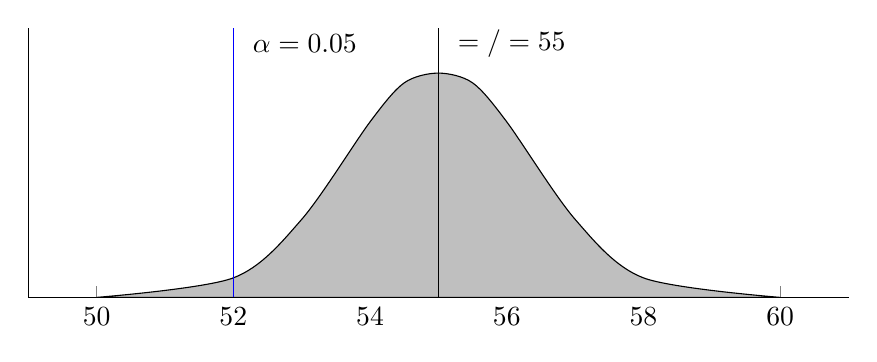
\begin{tikzpicture}
    \begin{axis}[
      axis lines*=left,
      ytick=\empty,
      height=5cm,
      width=12cm,
      enlarge y limits={value=0.2,upper},
      ]
      \addplot[smooth, fill=lightgray, domain=45:65] 
        coordinates{
          (50, 0) (52, 0.5) (53, 2) (54, 4.5) (54.5, 5.5)
          (55, 5.75)
          (55.5, 5.5) (56, 4.5) (57, 2) (58, 0.5) (60, 0)} 
        \closedcycle;

      \draw (55, 0) -- (55, 10);
      \node at (55, 6.5) [label=right:{$\populationmean = \HypPopMean/ = 55$}] {};

      \draw[color=blue] (52, 0) -- (52, 10);
      \node at (52, 6.5) [label=right:{$\alpha = 0.05$}] {};

    \end{axis}
  \end{tikzpicture}
\end{center}

\noindent
What we are doing here is we are making the non-rejection region smaller. Let's highlight the non-rejection region to see it:

\begin{center}
  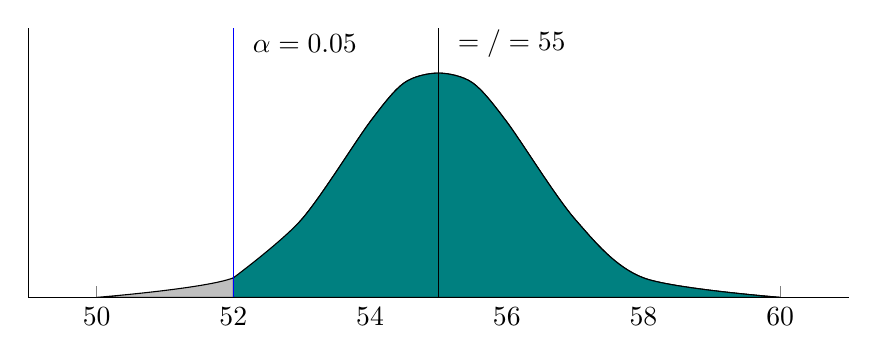
\begin{tikzpicture}
    \begin{axis}[
      axis lines*=left,
      ytick=\empty,
      height=5cm,
      width=12cm,
      enlarge y limits={value=0.2,upper},
      ]
      \addplot[smooth, fill=lightgray, domain=45:65] 
        coordinates{
          (50, 0) (52, 0.5) (53, 2) (54, 4.5) (54.5, 5.5)
          (55, 5.75)
          (55.5, 5.5) (56, 4.5) (57, 2) (58, 0.5) (60, 0)} 
        \closedcycle;

      \addplot[smooth, fill=teal, domain=45:65] 
        coordinates{
          (52, 0.5) (53, 2) (54, 4.5) (54.5, 5.5)
          (55, 5.75)
          (55.5, 5.5) (56, 4.5) (57, 2) (58, 0.5) (60, 0)} 
        \closedcycle;

      \draw (55, 0) -- (55, 10);
      \node at (55, 6.5) [label=right:{$\populationmean = \HypPopMean/ = 55$}] {};

      \draw[color=blue] (52, 0) -- (52, 10);
      \node at (52, 6.5) [label=right:{$\alpha = 0.05$}] {};

    \end{axis}
  \end{tikzpicture}
\end{center}

\noindent
We can see that there is a little tail on the left, in grey, that is in the rejection region (i.e., that is outside the non-rejection region). That area is the $\alpha$ area, which is 5\% of the total curve, because we chose to move the critical point up to that point.

Now suppose that we imagine another population mean, slid a little to the left. Let's call it $\populationmean_{1}$. So we're considering the true population mean, centered at 55, and another population mean, centered at 54:

\begin{center}
  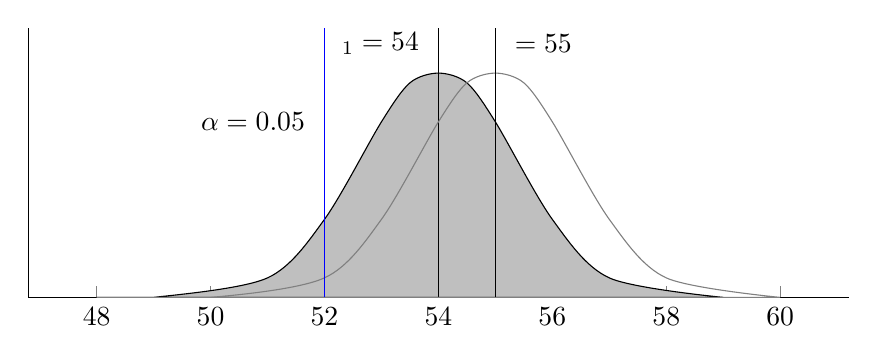
\begin{tikzpicture}
    \begin{axis}[
      axis lines*=left,
      ytick=\empty,
      height=5cm,
      width=12cm,
      enlarge y limits={value=0.2,upper},
      ]

      \addplot[smooth, fill=lightgray, domain=45:65] 
        coordinates{
          (48, 0)
          (49, 0) (51, 0.5) (52, 2) (53, 4.5) (53.5, 5.5)
          (54, 5.75)
          (54.5, 5.5) (55, 4.5) (56, 2) (57, 0.5) (59, 0)} 
        \closedcycle;

      \draw (54, 0) -- (54, 10);
      \node at (54, 6.5) [label=left:{$\populationmean_{1} = 54$}] {};

      \addplot[smooth, color=gray, domain=45:65] 
        coordinates{
          (48, 0)
          (50, 0) (52, 0.5) (53, 2) (54, 4.5) (54.5, 5.5)
          (55, 5.75)
          (55.5, 5.5) (56, 4.5) (57, 2) (58, 0.5) (60, 0)} 
        \closedcycle;

      \draw (55, 0) -- (55, 10);
      \node at (55, 6.5) [label=right:{$\populationmean = 55$}] {};

      \draw[color=blue] (52, 0) -- (52, 10);
      \node at (52, 4.5) [label=left:{$\alpha = 0.05$}] {};

    \end{axis}
  \end{tikzpicture}
\end{center}

\noindent
In the picture, we can see one sampling distribution where the mean is centered at 55, and another sampling distribution where the mean is centered at 54. We can also see $\alpha$, which is still marked at taking up 5\% of the curve centered at 55. 

Of course, we are looking at this through the eyes of an all-seeing God or Oracle here, because we can see that the real population mean is 55. If we put on our human analyst glasses, we do not know this. We only know that the sampling distribution centered around 54 is one possible sampling distribution amongst many, and the one centered around 55 is another possible sampling distribution amongst many.

Suppose now that we take a sample, and the mean of that sample is 51:

\begin{center}
  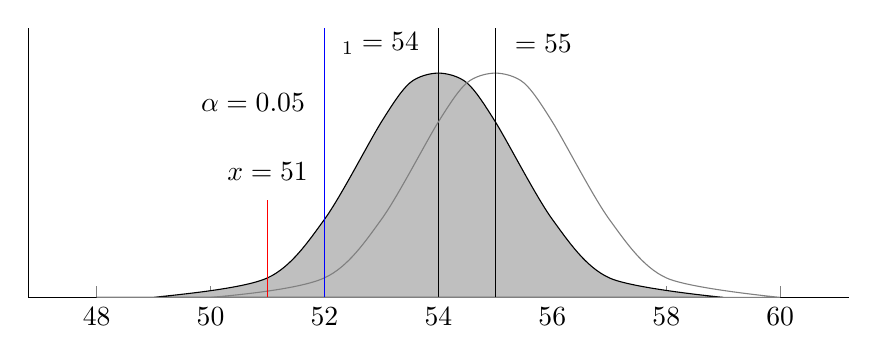
\begin{tikzpicture}
    \begin{axis}[
      axis lines*=left,
      ytick=\empty,
      height=5cm,
      width=12cm,
      enlarge y limits={value=0.2,upper},
      ]

      \addplot[smooth, fill=lightgray, domain=45:65] 
        coordinates{
          (48, 0)
          (49, 0) (51, 0.5) (52, 2) (53, 4.5) (53.5, 5.5)
          (54, 5.75)
          (54.5, 5.5) (55, 4.5) (56, 2) (57, 0.5) (59, 0)} 
        \closedcycle;

      \draw (54, 0) -- (54, 10);
      \node at (54, 6.5) [label=left:{$\populationmean_{1} = 54$}] {};

      \addplot[smooth, color=gray, domain=45:65] 
        coordinates{
          (48, 0)
          (50, 0) (52, 0.5) (53, 2) (54, 4.5) (54.5, 5.5)
          (55, 5.75)
          (55.5, 5.5) (56, 4.5) (57, 2) (58, 0.5) (60, 0)} 
        \closedcycle;

      \draw (55, 0) -- (55, 10);
      \node at (55, 6.5) [label=right:{$\populationmean = 55$}] {};

      \draw[color=blue] (52, 0) -- (52, 10);
      \node at (52, 5) [label=left:{$\alpha = 0.05$}] {};

      \draw[color=red] (51, 0) -- (51, 2.5);
      \node at (51, 2.5) [label=above:{$\samplemean{x} = 51$}] {};

    \end{axis}
  \end{tikzpicture}
\end{center}

\noindent
With our human analyst glasses on, we can't tell if this mean comes from the sampling distribution centered around 54, or from the one centered around 55. So what do we do? Do we reject, or accept the null hypothesis? 

Well, we are going to be strict and follow our procedure. Our procedure says that we will reject the null hypothesis if we get a sample mean that is below $\alpha$. And here, we do in fact have a sample mean that is below $\alpha$, so we will reject the null hypothesis.

However, when we step into the role of the all-seeing God or Oracle, we can see that the true population mean is centered at 55. And so, we have just rejected the null hypothesis, when we shouldn't have. We were mistaken. 

The sample we were looking at did not come from $\populationmean_{1}$. In truth, it came from $\populationmean$. But our $\alpha$ critical point threshold said we should reject the null hypothesis anyway.


%%%%%%%%%%%%%%%%%%%%%%%%%%%%%%%%%%%%%%%%%
%%%%%%%%%%%%%%%%%%%%%%%%%%%%%%%%%%%%%%%%%
\section{The probability of Type I Error}

As human analysts, we can never know if our judgment was correct or not. All \emph{we} know is that our sample mean fell below the threshold, and we therefore must reject the null hypothesis. Furthermore, since we cannot see the true population mean as an all-seeing God or Oracle could, we have no idea if we were right in rejecting the null hypothesis.

As human analysts, the best we can do is calculate the \emph{probability} of making this mistake. And what is the probability of mistakenly rejecting the null hypothesis? We can see here that it is exactly the area of $\alpha$, namely 0.05, or 5\%. The probability of making a Type I Error is exactly the amount of area that $\alpha$ cuts out of the sampling distribution centered at $\HypPopMean/$. 

So in this case, we can say the following. ``Well, we will never know if we did or did not make a mistake in rejecting the null hypothesis. But there is a 5\% chance that we were mistaken.''

In the example from the last section, we placed the critical point $\alpha$ exactly at the edge of the sampling distribution centered at $\HypPopMean/$. In that case, $\alpha$ cut out 0\% of that curve. And that is why we had a 0\% chance of committing a Type I Error in that example. 

Now, why not always set $\alpha$ at 0? Well, a 5\% chance is pretty small. So maybe we don't care that much about this kind of a mistake. Sure, we might mistakenly reject the null hypothesis, but only for 5\% of the samples that we could possible take. For 95\% of the samples that we could possibly take, we will not make a mistake.

On the other hand, sometimes you need really strict assurance, so you might set $\alpha$ at only 1\%. It depends on the hypothesis test. You, the analyst, get to set the $\alpha$ value, when you perform the hypothesis test.

Why do we call the critical point ``alpha''? Remember confidence intervals? There we said that $\alpha$ is the area outside of the confidence interval. If you have a confidence interval of 95\%, then $\alpha$ is 5\%. The $\alpha$ that we use here is exactly the same $\alpha$ that we use for confidence intervals.


\end{document}
